\documentclass[iop]{emulateapj}

\usepackage{tikz}
\usepackage{natbib}
\usepackage{amsmath}

\usetikzlibrary{shapes.geometric, arrows}
\usetikzlibrary{fit}

\tikzstyle{hyper} = [circle, text centered, draw=black]
\tikzstyle{param} = [circle, text centered, draw=black]
\tikzstyle{data} = [circle, text centered, draw=black, line width=2pt]
\tikzstyle{arrow} = [thick,->,>=stealth]

\usepackage{soul}
\usepackage[title]{appendix}

\newcommand{\myemail}{aimalz@nyu.edu}
\newcommand{\mathul}{\underline}
\newcommand{\chippr}{CHIPPR}
\newcommand{\nz}{$n(z)$}
\newcommand{\pz}{photo-$z$}
\newcommand{\pzpdf}{photo-$z$ PDF}


\begin{document}

\title{How to obtain the redshift distribution from probabilistic redshift 
estimates}%:\\

\author{Alex Malz\altaffilmark{1}}
\author{David W. Hogg\altaffilmark{1,2,3,4}}
\email{aimalz@nyu.edu}

\altaffiltext{1}{Center for Cosmology and Particle Physics, Department of 
Physics,
  New York University, 726 Broadway, 9th floor, New York, NY 10003, USA}
\altaffiltext{2}{Simons Center for Computational Astrophysics, 162 Fifth 
Avenue, 7th floor, New York, NY 10010, USA}
\altaffiltext{3}{Center for Data Science, New York University, 60 Fifth Avenue, 
7th floor, New York, NY 10003, USA}
\altaffiltext{4}{Max-Planck-Institut f\"ur Astronomie, K\"onigstuhl 17, D-69117 
Heidelberg, Germany}

\begin{abstract}
A trustworthy estimate of the redshift distribution $n(z)$ is crucial for 
weak-lensing cosmology as we know it.
Spectroscopic redshifts for the dim and numerous galaxies of weak-lensing 
surveys are expected to be inaccessible, making photometric redshifts 
(photo-$z$s) the next-best alternative.
The nontrivial systematics affecting photo-$z$ estimation have motivated the 
weak-lensing community to favor photo-$z$ probability density functions (PDFs) 
as a more comprehensive alternative to photo-$z$ point estimates.
However, analytic methods for utilizing these new data products in cosmological 
inference are still evolving.
The ubiquitous methodology known as stacking produces a systematically biased 
estimator of $n(z)$ that worsens with decreasing signal-to-noise, the very 
regime where photo-$z$ PDFs are most necessary.
We introduce a mathematically rigorous probabilistic graphical model (PGM) of 
hierarchical inference of $n(z)$, which is provably the only self-consistent 
way to combine photo-$z$ PDFs to produce an estimator of $n(z)$.
The novel Cosmological Hierarchical Inference with Probabilistic Photometric 
Redshifts (CHIPPR) model yields a more accurate characterization of $n(z)$ by 
correctly propagating the redshift uncertainty information beyond the best-fit 
estimator produced by traditional procedures.
We conclude by propagating these effects to constraints in the space of 
cosmological parameters.
\end{abstract}

\keywords{cosmology: cosmological parameters --- galaxies: statistics --- 
gravitational lensing: weak --- methods: data analysis --- methods: statistical}

\maketitle

\section{Introduction}
\label{sec:introduction}

\textcolor{blue}{Brief literature review addressing how \pzpdf s are currently 
used in cosmology}


\textcolor{blue}{Q: Why should we question existing methods?\\
A: Stacking is bad and only looks like it works because of assumptions that 
don't hold when the data is as bad as we anticipate.  Cite pedantic doc?}

overview of next questions: How can we improve the effectiveness of using 
\pzpdf s in inference?  How does the result of \chippr\ compare to established 
estimators in terms of the accuracy of \nz ?  \textcolor{blue}{Reach goal: How 
significant is the effect of the discrepancy between \nz\ estimators on 
cosmological constraints?}

\section{Methods}
\label{sec:methods}

\textcolor{blue}{Q: How can we improve the effectiveness of using \pzpdf s in 
inference?\\
A: Hierarchical inference is the only self-consistent way.}

This paper presents the Cosmological Hierarchical Inference with Probabilistic 
Photometric Redshifts (\chippr ) model as a mathematically consistent method 
for constraining \nz s using a catalog of \pzpdf s.
In Section~\ref{sec:model}, we introduce the \chippr\ formalism; in 
Section~\ref{sec:application}, we outline how to use \chippr\ to constrain \nz\ 
from a catalog of \pzpdf s; in Section~\ref{sec:limitations} we document the 
assumptions that must hold for \chippr\ to be valid.

\subsection{Model generalities}
\label{sec:model}

We begin by reframing the redshift distribution \nz\ from a probabilistic 
perspective.
Here we define a redshift distribution \nz\ as the normalized probability 
density
\begin{equation}
\label{eqn:nz}
\int_{-\infty}^{\infty}\ n(z)\ dz\ \equiv\ \frac{1}{J}\ 
\int_{-\infty}^{\infty}\ \sum_{j=1}^{J}\ \delta(z_{j},\ z)\ dz = 1
\end{equation}
of finding a galaxy $j$ in a catalog of $J$ galaxies having a redshift $z$.
We may without loss of generality impose a parametrization
\begin{equation}
\label{eqn:fz}
f_{\phi}(z)\ \equiv\ n(z)
\end{equation}
in terms of some parameter vector $\phi$.
We believe that galaxy redshifts are indeed drawn from \nz, making it a 
probability density over redshift; this fact can also be confirmed from 
dimensional analysis of Equation \ref{eqn:nz}.
Therefore, it can be rewritten as
\begin{equation}
\label{eqn:pz}
z_{j}\ \sim\ \Pr(z \mid \phi)\ \equiv\ f_{\phi}(z),
\end{equation}
a probability density over redshift conditioned on the parameters defining \nz.
Note that $z_{j}$ does not depend on $z_{j'}$, a statement of the causal 
independence of galaxy redshifts from one another.

In addition to believing \nz\ is a PDF from which redshifts are drawn, we also 
believe that there is some PDF from which photometric data $d$, which may be 
any combination of fluxes, magnitudes, colors, and their observational errors, 
are drawn.
Such a PDF over data is a likelihood
\begin{equation}
\label{eqn:pzpdf}
d\ \sim\ \Pr(d \mid z)
\end{equation}
conditioned on redshift.
This assumption that the data are drawn from some function of the redshift 
forms the foundation upon which \pz\ estimation is based.
Note that galaxies may have different observational data $d$ despite sharing 
the same redshift and that the data $d_{j}$ of one galaxy is causally 
independent of the redshifts $z_{j'}$ and data $d_{j'}$ of other galaxies.

This description of the physical system corresponds to a forward model by which 
we actually believe photometry is generated:
\begin{enumerate}
	\item There exists a redshift distribution \nz\ with parameters $\phi$.
	\item Galaxy redshifts $\{z_{j}\}$ are independent draws from $\Pr(z 
\mid \phi)$.
	\item Galaxy photometry $d_{j}$ is drawn from the likelihoods $\Pr(d | 
z_{j})$.
\end{enumerate}
A forward model such as this corresponds to a probabilistic graphical model 
(PGM), represented by a directed acyclic graph (DAG) as in Figure~\ref{fig:pgm}.
\begin{figure}
	\begin{center}
		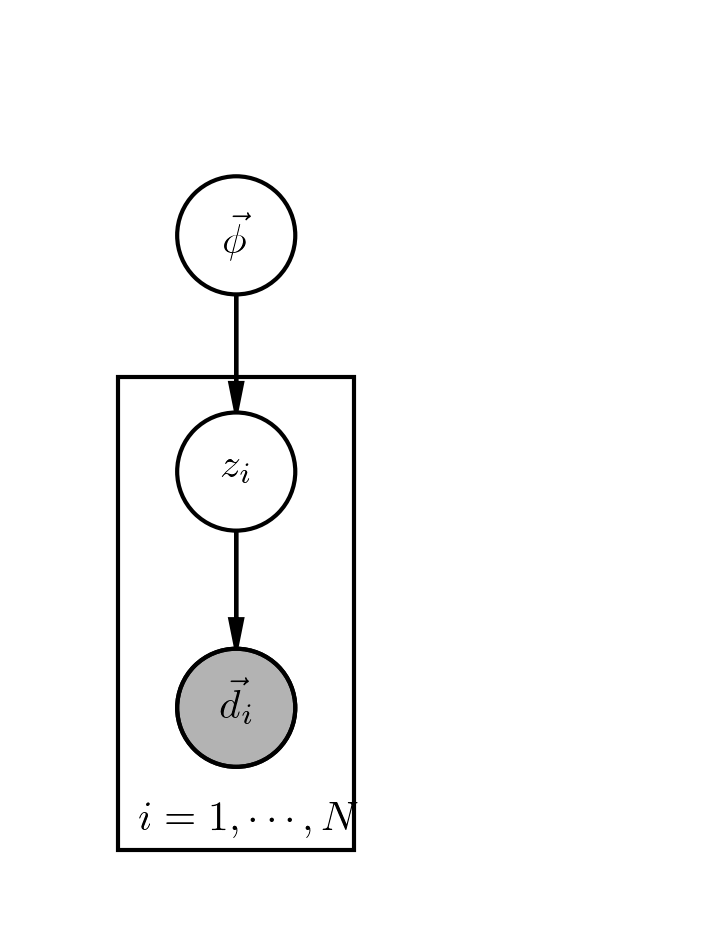
\includegraphics[width=0.25\textwidth]{fig/pgm.png}
		\caption{The PGM}
		\label{fig:pgm}
	\end{center}
\end{figure}
A DAG conveys the causal relationships between physical parameters and, like a 
Feynman diagram in the context of particle physics, is a shorthand for 
mathematical relationships between variables.

\subsection{Application to cosmology}
\label{sec:application}

The problem facing cosmologists is to determine the true parameters $\phi_{0}$ 
of \nz\ from observing the photometry $\{d_{j}\}$ of a large sample of galaxies 
$j$.
To self-consistently propagate the uncertainty in the redshifts, however, it is 
more appropriate to estimate the posterior $\Pr(\phi \mid \{d_{j}\})$ over all 
possible parameters $\phi$ (and thus potential redshift distributions \nz ) 
conditioned on all the observed data $\{d_{j}\}$ available in a generic catalog.

In order to use the DAG of Figure~\ref{fig:pgm} to derive an expression for 
$\Pr(\phi \mid \{d_{j}\})$ in terms of \pzpdf s, we must introduce two more 
concepts, confusingly named the implicit prior and the prior probability 
density.

When we constrain the redshift of a galaxy using its observed photometric data 
$d_{j}$, we are effectively estimating a posterior $\Pr(z \mid d_{j})$.
However, to do this, we must have a model for the general relationship between 
redshifts and photometry, whether empirical, as is the case for machine 
learning \pzpdf\ methods, or analytic, as is the case for template-based 
\pzpdf\ methods.
Such a relationship is defined in the space of probability density over 
redshift, so it must be able to be parameterized by the same functional form 
$f_{\phi}(z)$ as \nz .
It is thus natural to write it as $\Pr(z \mid \phi^{*})$, where $\phi^{*}$ is 
the parameters for this relationship under some generic \pzpdf\ method.
We call $\Pr(z \mid \phi^{*})$ the \textit{implicit prior}, as it is rarely 
explicitly known nor chosen by the researcher; for template-based methods where 
it can be chosen to be ``realistic,'' it may be appropriate to call it an 
\textit{interim prior}.
Because the implicit prior is unavoidable, the \pzpdf s reported by any method 
are really \textit{implicit-weighted posteriors} $\Pr(z \mid d, \phi^{*})$.

The prior probability density $\Pr(\phi)$ is a more familiar concept in 
astronomy; to progress, we will have to choose a prior probability density over 
all possible parameters $\phi$.
This prior need not be excessively proscriptive; for example, it may be chosen 
to enforce smoothness at physically motivated scales in redshift without 
imposing any particular region as over- or under-dense.

With these definitions, we obtain the desired expression for $\Pr(\phi \mid 
\{d_{j}\})$,
\begin{align}
\begin{split}
  \label{eqn:fullpost}
  \ln[\Pr(\phi \mid \{d_{j}\})] & \propto \ln[\Pr(\phi)] + \ln \left[\int dz 
\right.\\
  & \left. \exp \left[\sum_{j=1}^{J} \left(\ln[\Pr(z \mid d_{j}, \phi^{*})] 
\right. \right. \right.\\
  & \left. \left. \left. + \ln[\Pr(z \mid \phi)] - \ln[\Pr(z \mid \phi^{*})]\ 
\right)\ \right]\ \right] ,
\end{split}
\end{align}
which is the heart of \chippr.
The entire derivation of Equation~\ref{eqn:fullpost} is provided in 
Appendix~\ref{app:math}.

\subsection{Implementation}
\label{sec:implementation}

In this study, we compare the results of Equation~\ref{eqn:fullpost} to those 
of the two most common approaches to estimating \nz\ from a catalog of \pzpdf 
s: the distribution $n(z_{\mathrm{max}})$ of the redshifts at maximum posterior 
probability (i.e. the modes of the \pzpdf s), and the stacked estimator
\begin{align}
  \label{eqn:stacked}
  \hat{n}(z) &\equiv \frac{1}{J}\ \sum_{j=1}^{J}\ \Pr(z \mid d_{j}, \phi^{*}) .
\end{align}

We perform this comparison on mock data in the form of catalogs of emulated 
\pzpdf s generated via the forward model discussed above and presented in 
detail in Appendix~\ref{app:data}.
The mock data emulates the three sources of error of highest concern to the 
\pz\ community: intrinsic scatter, catastrophic outliers, and systematic bias.
Figure~\ref{fig:mega_scatter} illustrates these three effects individually at 
ten times the tolerance of the upcoming Large Synoptic Survey Telescope (LSST).
\begin{figure*}
	\begin{center}
		
\includegraphics[width=0.3\textwidth]{fig/forward_model_example.png}
    \includegraphics[width=0.3\textwidth]{fig/forward_model_example.png}
    \includegraphics[width=0.3\textwidth]{fig/forward_model_example.png}
		\caption{Show this for each individually.}
		\label{fig:mega_scatter}
	\end{center}
\end{figure*}
Tests including all three effects at the tolerance levels of LSST and at twice 
the tolerance levels of LSST are presented in Section~\ref{sec:results}.

\subsection{Limitations}
\label{sec:limitations}

Finally, we explicitly review the assumptions made by this approach.
\begin{itemize}
  \item prior $\Pr(\phi)$
  \item implicit prior $\phi^{*}$ known
	\item \pzpdf s are accurate posteriors %draws from photo-$z$ PDFs do 
not match marginal distributions in $z_true$ vs. $z_phot$ space, i.e. toy model 
with $z_phot$ drawn from an uglier space but pdfs evaluated in lsst-limits space
	\end{itemize}






\section{Results}
\label{sec:results}

\textcolor{blue}{Q: How does the result of \chippr compare to established 
estimators in terms of the accuracy of $n(z)$?\\
A: \chippr yields the best possible $n(z)$, conditional on the accuracy of the 
photo-$z$ PDFs used.}

\subsection{Idealized example}
\label{sec:idealized}

\textcolor{blue}{LSST specs: unbiased, uniform outliers, medium z-dependent 
scatter}

\begin{figure*}
	\begin{center}
		
\includegraphics[width=0.45\textwidth]{fig/forward_model_example.png}
		\includegraphics[width=0.45\textwidth]{fig/results_example.png}
		\caption{Show this for idealized case.}
		\label{fig:idealized}
	\end{center}
\end{figure*}

\subsection{Realistic example}
\label{sec:realistic}

\textcolor{blue}{DES(?) specs: biased to enhance true $n(z)$, systematic 
outliers, high z-dependent scatter}

\begin{figure*}
	\begin{center}
		
\includegraphics[width=0.45\textwidth]{fig/forward_model_example.png}
		\includegraphics[width=0.45\textwidth]{fig/results_example.png}
		\caption{Show this for realistic case.}
		\label{fig:realistic}
	\end{center}
\end{figure*}

\subsection{Violations of the model}
\label{sec:violations}

\textcolor{blue}{mischaracterized interim prior, with idealized or realistic 
data?}

\begin{figure*}
	\begin{center}
		
\includegraphics[width=0.45\textwidth]{fig/forward_model_example.png}
		\includegraphics[width=0.45\textwidth]{fig/results_example.png}
		\caption{Show this for mischaracterized case.}
		\label{fig:mischaracterized}
	\end{center}
\end{figure*}


\section{Discussion}
\label{sec:discussion}



\section{Conclusion}
\label{sec:conclusion}

\section*{Appendices}

\begin{appendices}

\section{Mathematical derivation}
\label{app:math}

\section{Mock data generation}
\label{app:data}

\textul{Plots: flow chart of forward model}

\begin{figure*}
	\begin{center}
		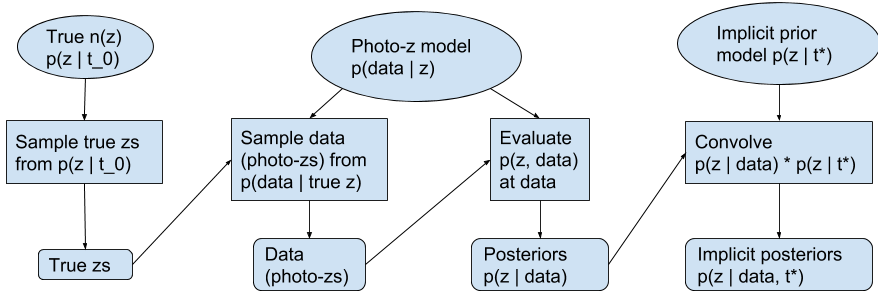
\includegraphics[width=0.75\textwidth]{fig/flowchart.png}
		\caption{In appendix?}
		\label{fig:flowchart}
	\end{center}
\end{figure*}


\end{appendices}

\begin{acknowledgements}
AIM thanks Elisabeth Krause for assistance with the \texttt{CosmoLike} code, 
Mohammadjavad Vakili for insightful input on statistics, Geoffrey Ryan for 
advice on debugging, and Boris Leistedt for helpful comments provided in the 
preparation of this paper.
This work was completed under the generous nutritional support of the Center 
for Computational Astrophysics.
\end{acknowledgements}

\bibliographystyle{apj}
\bibliography{references}

\end{document}
